\section{مقدمه}

در این تمرین، یک واحد حساب و منطق (\lr{ALU}) ترکیبی 32 بیتی را طراحی کردیم که می‌تواند عملیات جمع، تفریق و ضرب را انجام دهد. مطابق صورت تمرین، ورودی‌ها و خروجی‌های این واحد به این صورت هستند:
\begin{itemize}
    \item \textbf{ورودی:}
          \begin{enumerate}
              \item \textbf{\lr{\code{A}}}: عملوند اول (32 بیت)
              \item \textbf{\lr{\code{B}}}: عملوند دوم (32 بیت)
              \item \textbf{{\lr{\code{ALU\_Ctrl}}}}: سیگنال کنترلی تعیین نوع علامت (3 بیت)
          \end{enumerate}

    \item \textbf{خروجی:}
          \begin{enumerate}
              \item \textbf{\lr{\code{Result\_Lo}}}: 32 بیت کم‌ارزش حاصل عملیات (32 بیت)
              \item \textbf{\lr{\code{Result\_Hi}}}: 32 بیت پرارزش حاصل عملیات (تنها در عملیات ضرب کاربرد دارد) (32 بیت)
              \item \textbf{\lr{\code{C (Carry)}}}: پرچم رقم نقلی (1 بیت)
              \item \textbf{\lr{\code{V (Overflow)}}}: پرچم سرریز (1 بیت)
              \item \textbf{\lr{\code{Z (Zero)}}}: پرچم صفر (1 بیت)
              \item \textbf{\lr{\code{N (Negative)}}}: پرچم منفی (1 بیت)
          \end{enumerate}
\end{itemize}

و خروجی‌ها نیز به ازای عملیات مختلف به این صورت هستند:

\begin{table}[H]
    \centering
    \caption{کدهای کنترلی واحد حساب و منطق}
    \vspace{0.2cm}
    \begin{tabular}{|c|c|c|c|}
        \hline
        \textbf{کد کنترلی} & \textbf{نام دستور} & \textbf{شرح عملیات}                         & \textbf{پرچم‌های فعال} \\
        \hline
        $000$              & \lr{ADD\_U}        & جمع دو عدد بدون علامت ($A + B$)             & \lr{C, Z, V}          \\
        \hline
        $001$              & \lr{ADD\_S}        & جمع دو عدد علامت‌دار ($A + B$)               & \lr{V, N, Z}          \\
        \hline
        $010$              & \lr{SUB\_U}        & تفریق دو عدد بدون علامت ($A - B$)           & \lr{C, Z, V}          \\
        \hline
        $011$              & \lr{SUB\_S}        & تفریق دو عدد علامت‌دار ($A - B$)             & \lr{V, N, Z}          \\
        \hline
        $100$              & \lr{MUL\_U}        & ضرب ترکیبی دو عدد بدون علامت ($A \times B$) & \lr{Z}                \\
        \hline
        سایر حالت‌ها        & \lr{NOP}           & خروجی‌ها صفر باشند.                          & هیچ‌کدام               \\
        \hline
    \end{tabular}
\end{table}

\pagebreak

\section{عملیات جمع و تفریق}
جمع‌کننده به صورت انتشار رقم نقلی (\lr{Carry Ripple Adder}) و تفریق‌کننده نیز به صورت جمع متمم دو پیاده‌سازی شد.

ابتدا، یک جمع‌کننده کامل (\lr{Full Adder} یا به اختصار \lr{FA}) ساختیم:
\begin{figure}[H]
    \centering
    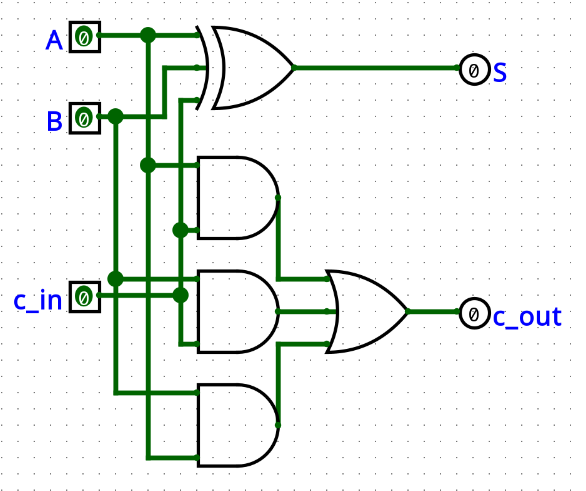
\includegraphics[width=0.4\textwidth]{assets/FA.png}
    \caption{جمع‌کننده کامل (\lr{FA})}
\end{figure}

سپس با کنار هم قرار دادن 8 واحد \lr{FA}، یک جمع‌کننده/تفریق‌کننده 8 بیتی ساختیم: با استفاده از ابزار \lr{Splitter} در \lr{Logisim}، بیت‌های دو ورودی 8 بیتی \lr{A} و \lr{B} را جدا کردیم. بیت‌های \lr{A} مستقیم به ورودی اول \lr{FA} ها وصل شدند. بیت‌های \lr{B} نیز با ورودی تک‌بیتی \lr{sub}، \code{XOR} شده و سپس به ورودی دیگر جمع‌کننده‌ها رفتند. همچنین ورودی تک‌بیتی \lr{c\_in} به ورودی \lr{c\_in} جمع‌کننده اول وصل شد. سپس، \lr{c\_out} هر جمع‌کننده را به ورودی \lr{c\_in} جمع‌کننده بعدی وصل کردیم. \\
با استفاده از \lr{Splitter}، خروجی \lr{S}ِ جمع‌کننده‌ها را کنار هم قرار دادیم تا یک خروجی 8 بیتی ساخته شود. \lr{c\_out} جمع‌کننده‌ی آخر نیز همان خروجی \lr{c\_out} مدار است:

\begin{figure}[H]
    \centering
    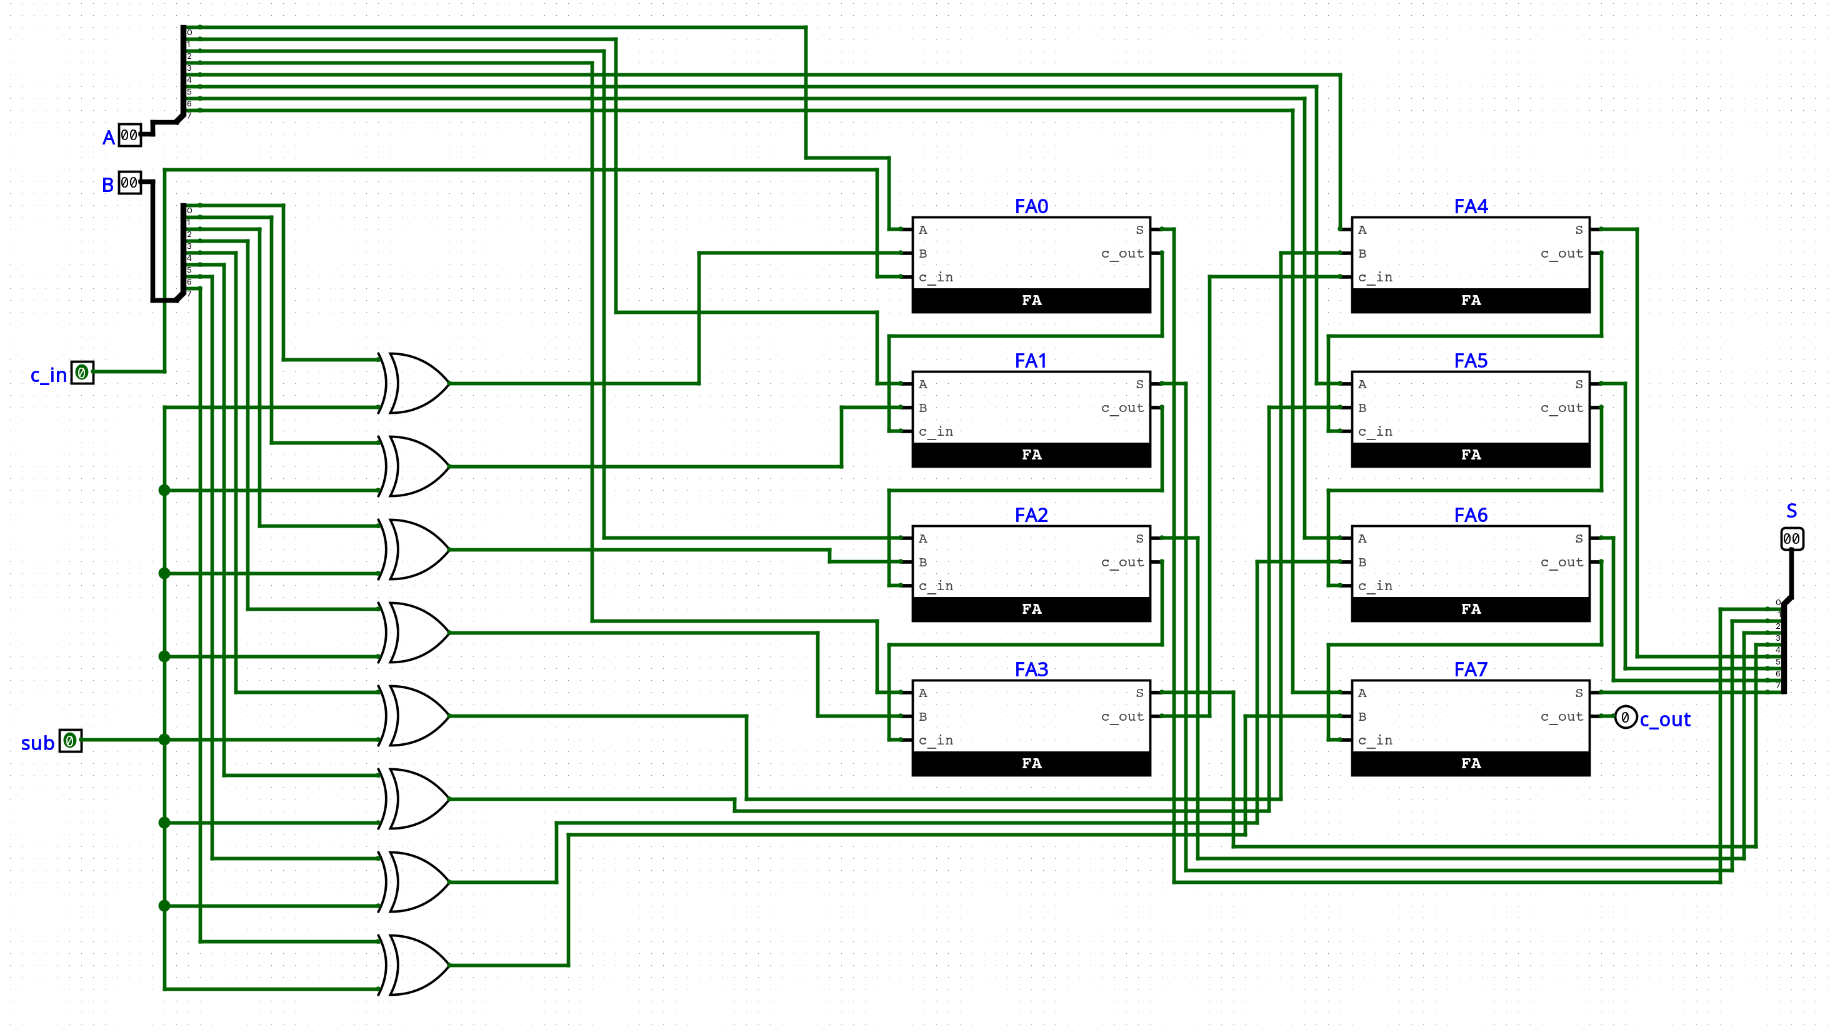
\includegraphics[width=0.9\textwidth]{assets/8bit_rcas.png}
    \caption{جمع‌/تقریق کننده 8 بیتی}
\end{figure}

با \code{XOR} کردن ورودی \lr{sub} با بیت‌های \lr{B}، عملیات تفریق با استفاده از مکمل دو (\lr{Two's Complement}) انجام می‌شود؛ با \code{XOR} کردن، مکمل یک \lr{B} ساخته می‌شود (\lr{$\overline{B}$})، سپس همان طور که در بخش بعدی می‌بینیم، چون \lr{sub} را به ورودی \lr{c\_in} جمع/تفریق کننده‌ی اول نیز وصل کردیم، ورودی‌ها با 1 جمع شده و فرمول زیر اجرا می‌شود:
\begin{align*}
    A - B = A + (-B) = A + \overline{B} + 1
\end{align*}

برای ساخت جمع/تفریق کننده‌ی 32 بیتی، به طور مشابه 4 واحد از جمع/تفریق کننده‌های 8 بیتی را کنار هم قرار دادیم. بیت‌های دو وردی 32 بیتی \lr{A} و \lr{B} را به 4 بخش 8 بیتی تبدیل کرده و به هر یک از چهار پیمانه (\lr{module}) دادیم. ورودی \lr{sub} نیز به \lr{c\_in}ِ پیمانه‌ی اول و \lr{sub}ِ هر چهار پیمانه متصل شد. \\
خروجی‌ها نیز مشابه بخش قبلی هستند:

\begin{figure}[H]
    \centering
    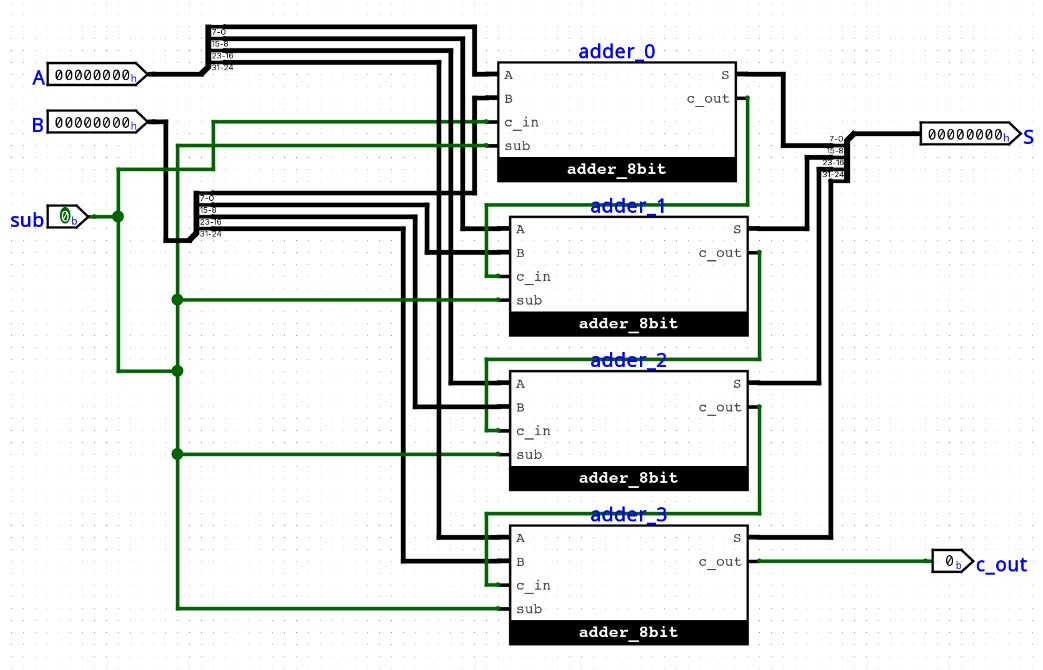
\includegraphics[width=0.9\textwidth]{assets/32bit_rcas.png}
    \caption{جمع‌/تقریق کننده 32 بیتی}
\end{figure}

در نهایت، واحد جمع/تفریق کننده (که آن را \code{adder\_32bit} می‌نامیم) به این صورت است:

\begin{figure}[H]
    \centering
    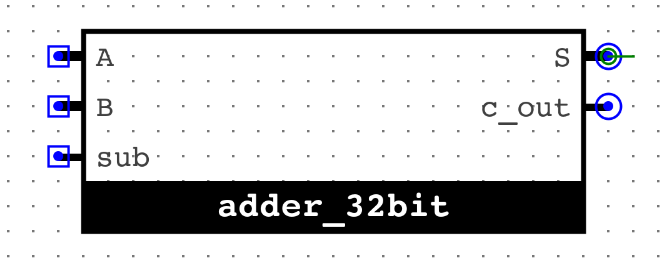
\includegraphics[width=0.5\textwidth]{assets/adder_32bit.png}
    \caption{پیمانه‌ی \code{adder\_32bit}}
\end{figure}

\pagebreak

\section{عملیات ضرب}
ابتدا یک ضرب‌کننده‌ی 4 بیتی ترکیبی را به این صورت ساختیم: (در این مرحله علاوه بر \lr{FA} که در بخش قبل ساخته بودیم، از \lr{Half Adder (HA)} هم استفاده کردیم)

\begin{figure}[H]
    \centering
    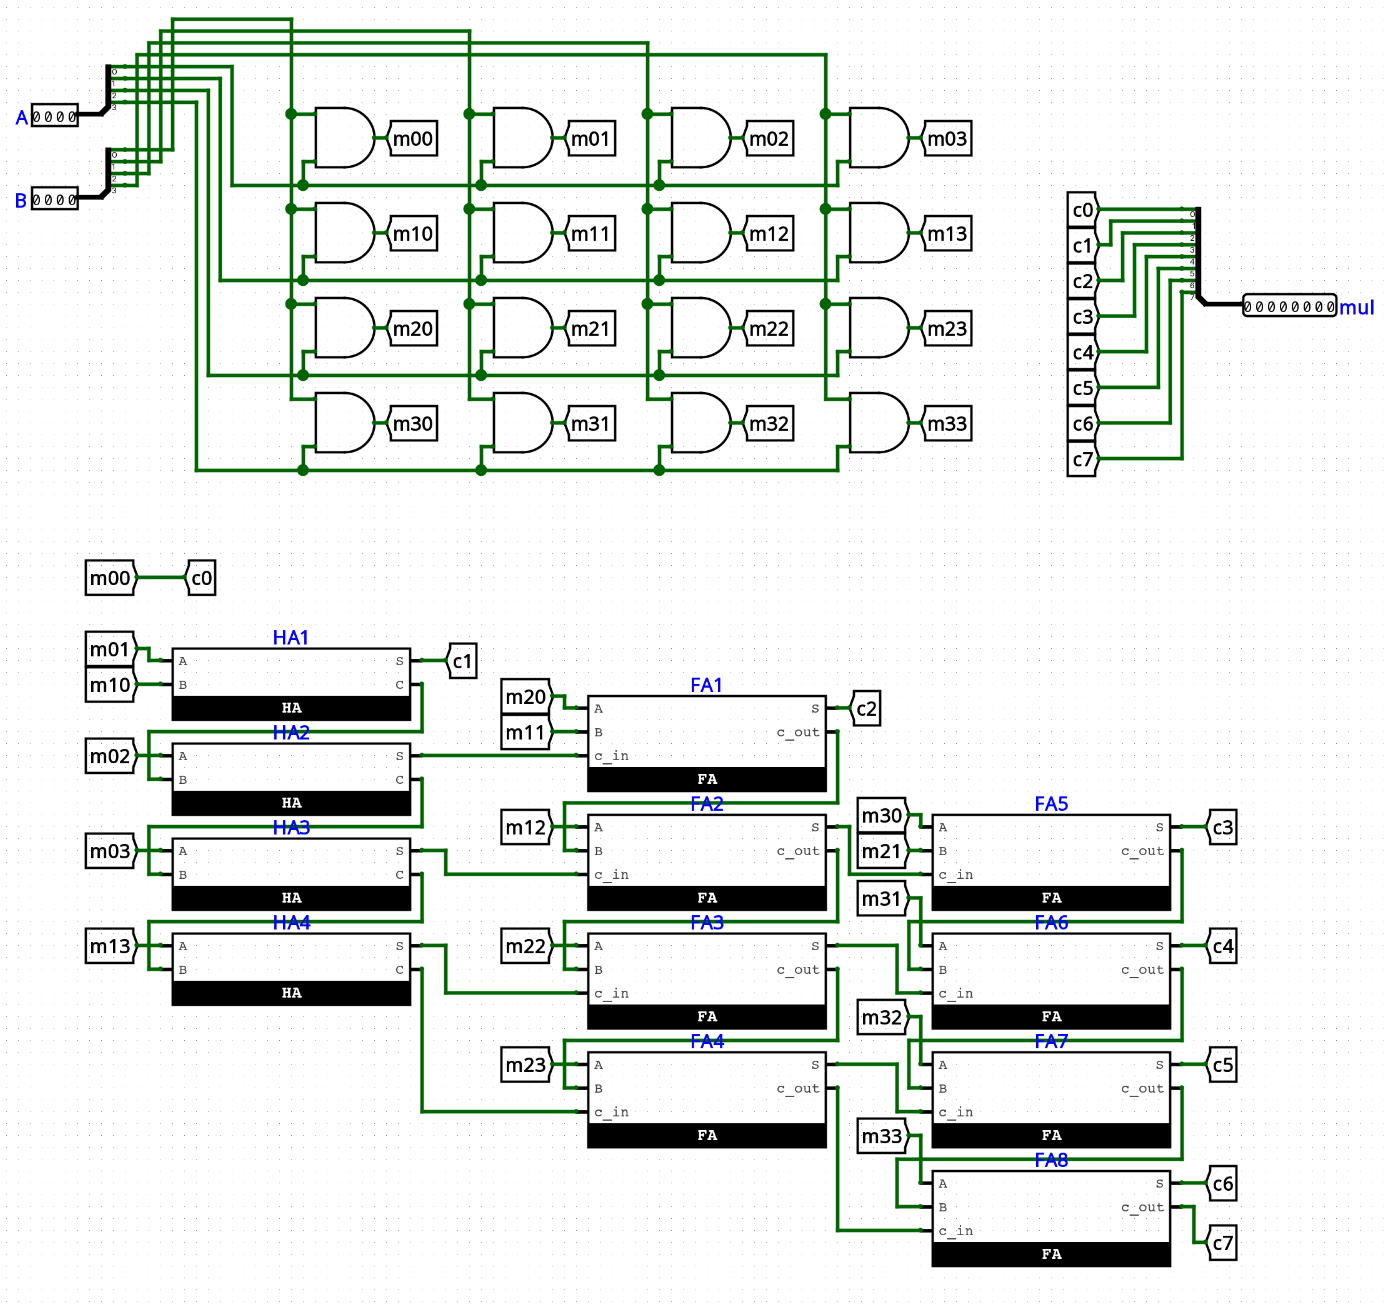
\includegraphics[width=0.6\textwidth]{assets/mul_4bit.png}
    \caption{ضرب‌کننده‌ی ترکیبی 4 بیتی}
\end{figure}

سپس، سعی کردیم با قرار دادن چهار واحد از ضرب‌کننده‌های 4 بیتی کنار هم و با استفاده از الگوریتم تقسیم و غلبه (\lr{Divide and Conquer})، ضرب‌کننده‌ی 8 بیتی بسازیم. از نظر ریاضی، اگر دو عدد 8 بیتی $A$ و $B$ را به دو بخش 4 بیتی کم‌ارزش (\lr{Low}) و پرارزش (\lr{High}) تقسیم کنیم، عملیات ضرب به شکل زیر بسط داده می‌شود:
\begin{align*}
    A          & = A_H \cdot 2^4 + A_L                                                           \\
    B          & = B_H \cdot 2^4 + B_L                                                           \\
    A \times B & = (A_H \cdot 2^4 + A_L) \times (B_H \cdot 2^4 + B_L)                            \\
               & = (A_H \times B_H)2^8 + (A_H \times B_L + A_L \times B_H)2^4 + (A_L \times B_L)
\end{align*}

بر اساس این منطق، مدار ضرب‌کننده‌ی 8 بیتی به شکل زیر پیاده‌سازی شده است:
\begin{figure}[H]
    \centering
    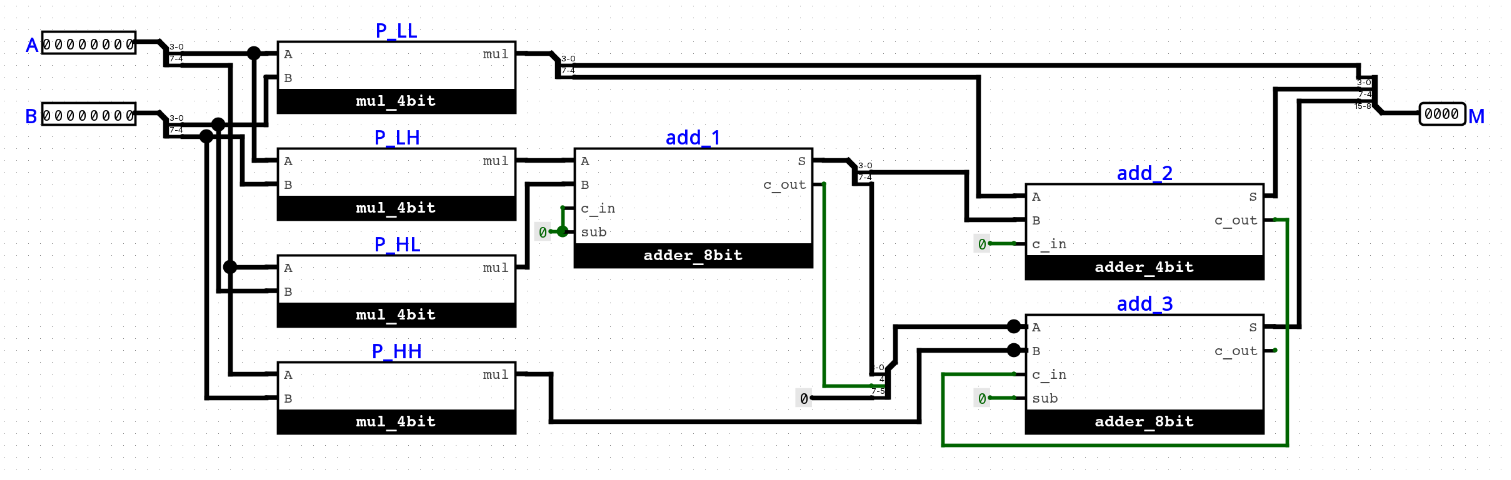
\includegraphics[width=0.8\textwidth]{assets/mul_8bit.png}
    \caption{ضرب‌کننده‌ی ترکیبی 8 بیتی}
\end{figure}

همان‌طور که در تصویر مشخص است، روند اجرای مدار شامل مراحل زیر است:
\begin{itemize}
    \item \textbf{جداسازی ورودی‌ها:} ابتدا با استفاده از ماژول \lr{Splitter}، ورودی‌های 8 بیتی $A$ و $B$ هر کدام به دو بخش 4 بیتی تقسیم می‌شوند.
    \item \textbf{حاصل‌ضرب‌های جزئی:} این بخش‌ها به چهار واحد ضرب‌کننده‌ی 4 بیتی وارد می‌شوند تا چهار حاصل‌ضرب جزئی (\lr{P\_LL, P\_LH, P\_HL, P\_HH}) تولید شود.
    \item \textbf{جمع و شیفت:}
          \begin{itemize}
              \item با استفاده از یک جمع‌کننده‌ی 8 بیتی (\lr{add\_1})، عبارات میانی ($P_{LH} + P_{HL}$) با هم جمع می‌شوند.
              \item 4 بیت کم‌ارزش خروجی $P_{LL}$ مستقیماً به عنوان 4 بیت اولِ خروجی نهایی استفاده می‌شود. 4 بیت پرارزش آن به کمک یک جمع‌کننده‌ی 4 بیتی (\lr{add\_2}) با 4 بیت کم‌ارزشِ حاصل‌جمع میانی (\lr{add\_1}) جمع شده و 4 بیت دوم خروجی نهایی را می‌سازد.
              \item در نهایت، یک جمع‌کننده‌ی 8 بیتی دیگر (\lr{add\_3})، حاصل‌ضرب پرارزش ($P_{HH}$) را با بخش‌های باقی‌مانده از جمع‌های قبلی (همراه با لحاظ کردن رقم نقلی یا \lr{c\_out} از \lr{add\_2} به عنوان \lr{c\_in} و همچنین \lr{c\_out} بلوک \lr{add\_1}) جمع می‌کند تا 8 بیت پرارزش نهایی تولید شود.
          \end{itemize}
    \item \textbf{الحاق خروجی‌ها:} در انتها، با استفاده مجدد از یک \lr{Splitter} (به صورت معکوس)، بخش‌های محاسبه‌شده با یکدیگر ترکیب (الحاق) می‌شوند تا خروجی نهایی 16 بیتی (\lr{M}) ساخته شود.
\end{itemize}

سپس به طریق کاملاً مشابه، از این پیمانه استفاده کردیم تا ضرب‌کننده‌ی 16 بیتی بسازیم و به کمک آنها هم ضرب‌کننده‌ی 32 بیتی ساخته شد:
\begin{figure}[H]
    \centering
    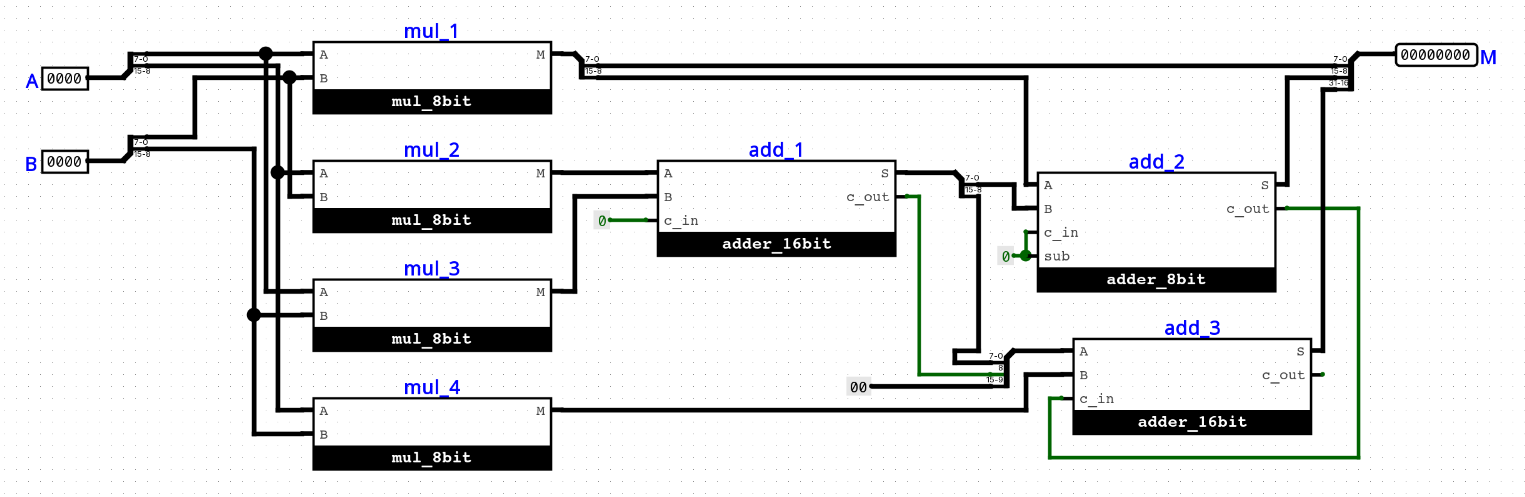
\includegraphics[width=0.8\textwidth]{assets/mul_16bit.png}
    \caption{ضرب‌کننده‌ی ترکیبی 16 بیتی}
\end{figure}

\begin{figure}[H]
    \centering
    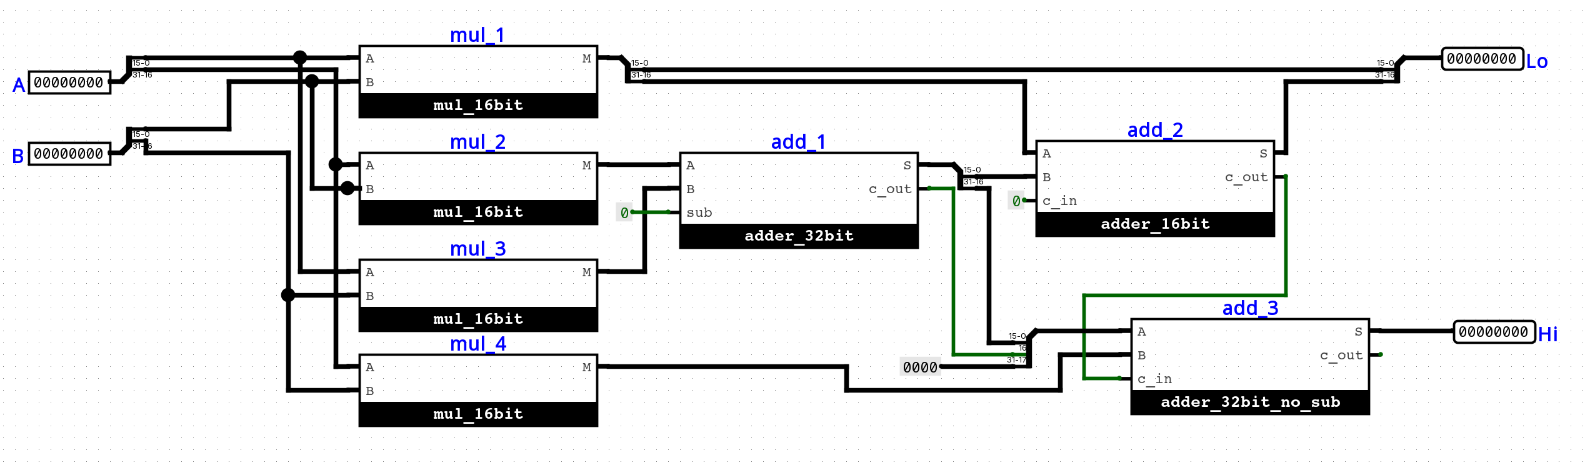
\includegraphics[width=0.8\textwidth]{assets/mul_32bit.png}
    \caption{ضرب‌کننده‌ی ترکیبی 32 بیتی}
\end{figure}

\pagebreak

در نهایت، واحد ضرب‌کننده (که آن را \code{mul\_32bit} می‌نامیم) به این صورت است:
\begin{figure}[H]
    \centering
    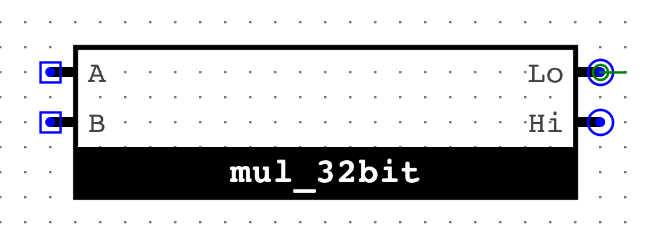
\includegraphics[width=0.5\textwidth]{assets/mul_32bit_module.png}
    \caption{پیمانه‌ی \code{mul\_32bit}}
\end{figure}

\pagebreak

\section{واحد حساب و منطق (\code{ALU})}
مدار طراحی شده‌ی این قسمت به این صورت است:
\begin{figure}[H]
    \centering
    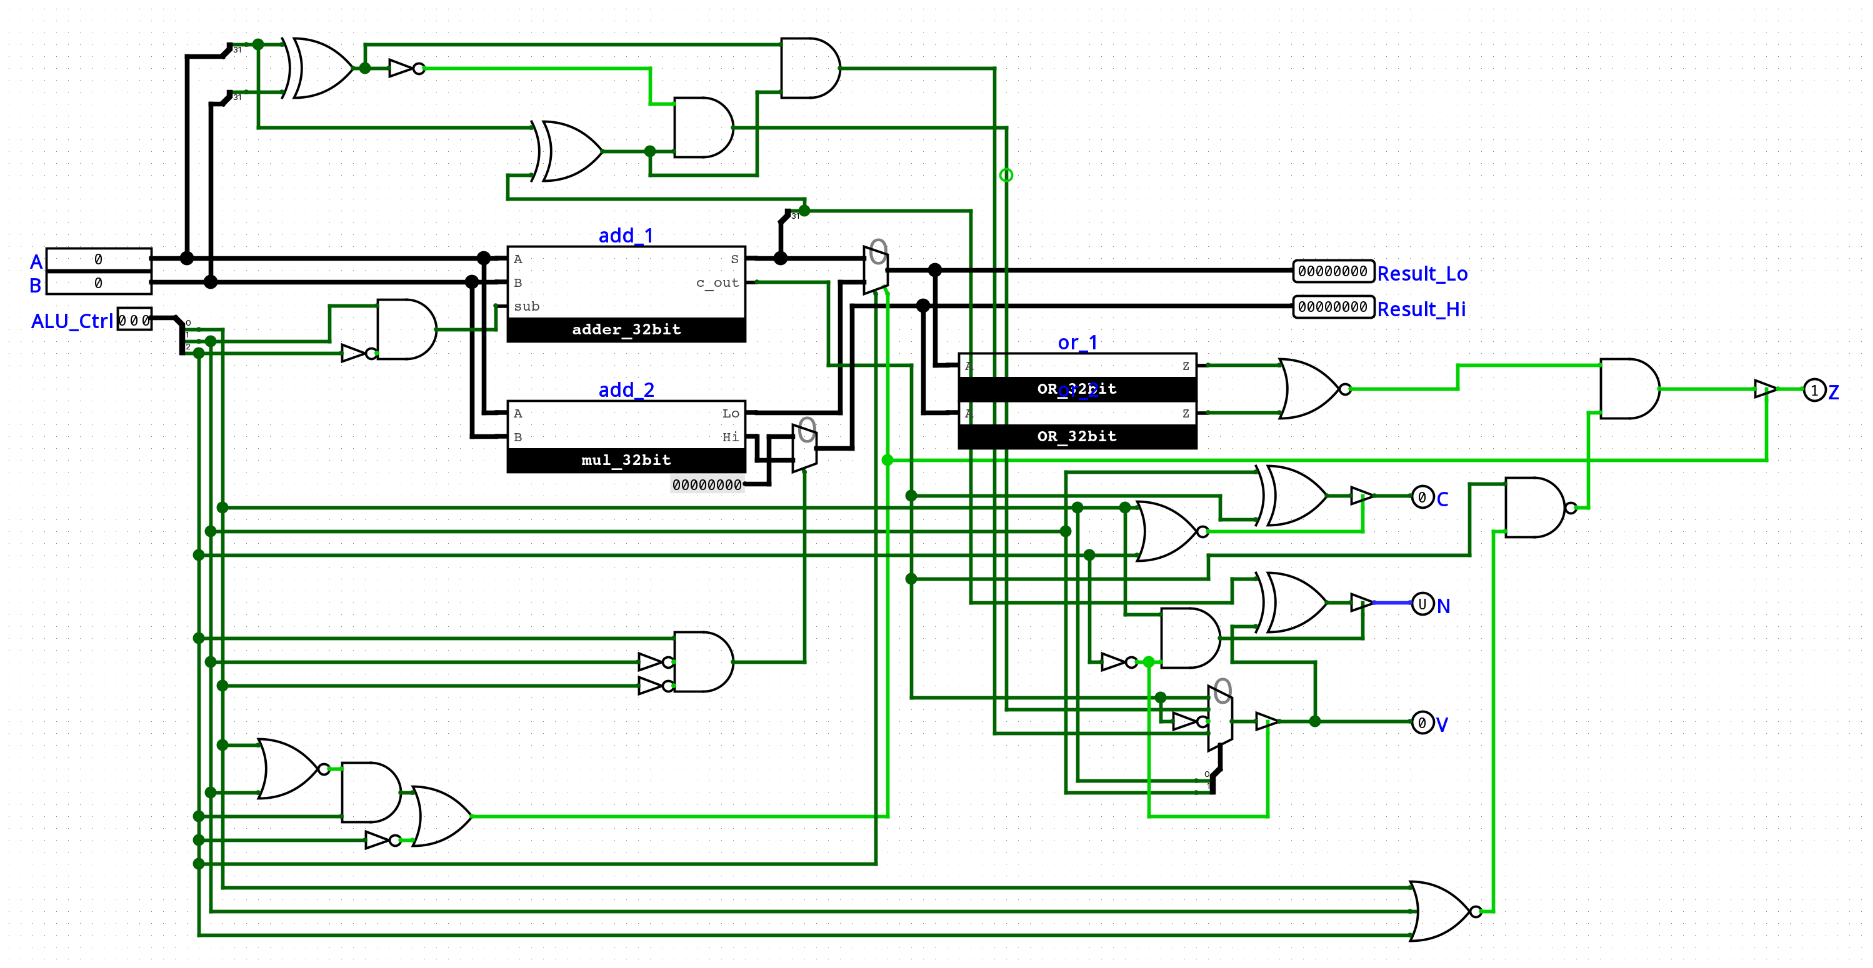
\includegraphics[width=1.0\textwidth]{assets/ALU_32bit.png}
    \caption{واحد حساب و منطق 32 بیتی}
\end{figure}

در ادامه، هر بخش را جداگانه توضیح می‌دهیم.

\subsection{تولید خروجی‌ها (مسیر داده)}
ورودی‌های 32 بیتی \lr{A} و \lr{B} را هم‌زمان به ورودی‌های پیمانه‌ی \code{adder\_32bit} و \code{mul\_32bit} می‌دهیم تا هر دو عملیات به موازات هم انجام شوند (تفاوت بین حالت‌های جمع و تفریق در بخش بعد توضیح داده می‌شود).

دو مالتی‌پلکسر (\lr{MUX}) دو به یک در مدار قرار داده (\lr{bitwidth}ِ هر دو 32 بیت است) و خروجی‌های آن‌ها را به ترتیب \code{Result\_Lo} و \code{Result\_Hi} می‌نامیم. خروجی اصلیِ واحد جمع‌کننده و خروجی \lr{Lo}ِ ضرب‌کننده به مالتی‌پلکسر اول متصل شده‌اند تا \code{Result\_Lo} را تشکیل دهند. خروجی \lr{Hi}ِ ضرب‌کننده نیز به ورودیِ یکِ مالتی‌پلکسر دوم وصل شده و ورودی دیگرِ آن به مقدار ثابت صفر وصل شده تا \code{Result\_Hi} را کنترل کند.

\subsection{رمزگشایی کد کنترل}
سیگنال کنترلی \code{ALU\_Ctrl} (که آن را به اختصار \lr{AC} می‌نامیم) سه بیت دارد: بیت پرارزش ($AC_2$) نوع عملیات پایه (جمع/تفریق یا ضرب) را مشخص می‌کند؛ بیت میانی ($AC_1$) جمع یا تفریق بودن را تعیین می‌کند؛ و بیت کم‌ارزش ($AC_0$) نیز بی‌علامت یا علامت‌دار بودن عملیات را مشخص می‌سازد.

در حالت $\text{\lr{AC}}_2 = 0$، باید خروجی مدار جمع/تفریق کننده در \code{Result\_Lo} نوشته شود، بنابراین این بیت را به خط انتخاب (\lr{select}) مالتی‌پلکسر اول وصل می‌کنیم. همچنین خروجی \code{Result\_Hi} تنها در حالت $\text{\lr{AC}} = 100$ فعال بوده و در حالت‌های دیگر صفر است. بنابراین به کمک یک گیت \code{AND} و گیت‌های \code{NOT}، مقدار ${AC}_2\overline{{AC}_1{AC}_0}$ را ساخته و به خط انتخاب مالتی‌پلکسر دیگر وصل می‌کنیم.

برای کنترل عملگر جمع یا تفریق، سیگنال $\overline{AC_2}AC_1$ تولید شده و به ورودی \lr{sub} در پیمانه‌ی جمع‌کننده متصل شده است تا در صورت صدور دستورات تفریق ($AC_2AC_1 = 01$)، مدار به صورت مکملِ دو عمل کند.

\subsection{تولید پرچم‌ها (Flags)}
خروجی هر یک از پرچم‌ها توسط یک بافر سه‌حالته (\lr{Tri-state Buffer}) کنترل می‌شود تا پرچم‌ها تنها در دستوراتی که از نظر منطقی معتبر هستند خروجی دهند و در سایر حالت‌ها در وضعیت امپدانس بالا (\lr{High Impedance}) قرار گیرند. معادلات فعال‌ساز (\lr{Enable}) و منطق محاسبه‌ی هر پرچم بر اساس مدار به شرح زیر است:

\begin{align*}
    C & = AC_1 \oplus \text{\code{c\_out}}                                                                                                                                    \\
    \\
    V & = (\overline{AC_1AC_0})(\text{\code{c\_out}}) + (\overline{AC_1}AC_0)((A_{31} \odot B_{31}) \cdot (A_{31} \oplus S_{31}))                                             \\
      & + ({AC_1}\overline{AC_0})(\overline{\text{\code{c\_out}}}) + ({AC_1AC_0})((A_{31} \oplus B_{31}) \cdot (A_{31} \oplus S_{31}))                                        \\
    \\
    Z & = (\text{OR}(\text{\code{Result\_Lo}}) \downarrow \text{OR}(\text{\code{Result\_Hi}})) \cdot ((\text{\code{c\_out}}) \uparrow (AC_2 \downarrow AC_1 \downarrow AC_0)) \\
    \\
    N & = S_{31} \oplus V
\end{align*}

در نهایت، واحد محاسبه و منطق (که آن را \code{ALU\_32bit} می‌نامیم) به این صورت است:

\begin{figure}[H]
    \centering
    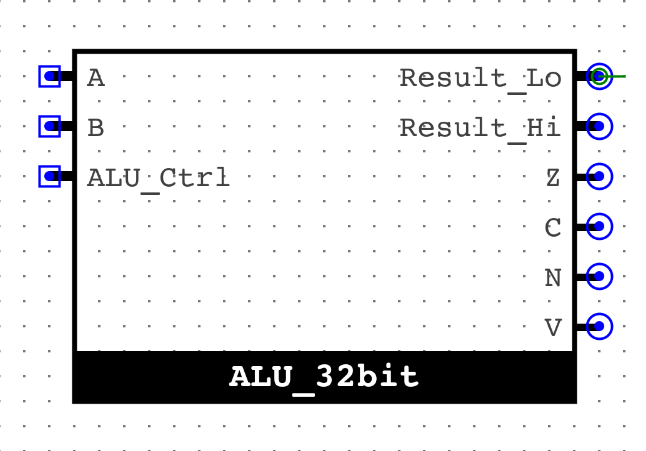
\includegraphics[width=0.6\textwidth]{assets/ALU_32bit_module.png}
    \caption{پیمانه‌ی \code{ALU\_32bit}}
\end{figure}

\pagebreak

\section{اجرای آزمون}
به کمک اسکریپت‌های داده شده، مدار را سنتز کرده و تست‌ها را اجرا می‌کنیم. نتیجه‌ی آزمون به این صورت است که موفقیت‌آمیز بودن تمامی عملیات‌ها را تایید می‌کند: \\

\begin{latin}
    \begin{lstlisting}[basicstyle=\ttfamily\small, breaklines=true, postbreak=\mbox{\textcolor{red}{$\hookrightarrow$}\space}]
mohsen@Quanta:/mnt/D/SUT/Term_4/CA/ca4042-judge$ ./validate.sh ./HW1/tb.v ~/logisim_evolution_workspace/HW1_403106238.circ.tmp/HW1_403106238.circ.tmp
./HW1/tb.v:34: Warning: Calling system function $random() as a task.
./HW1/tb.v:34:          The functions return value will be ignored.
ADD_U
SUB_U
ADD_S
SUB_S
MUL_U
ACCEPTED
         50 /         50
mohsen@Quanta:/mnt/D/SUT/Term_4/CA/ca4042-judge$ 
\end{lstlisting}
\end{latin}
